\vzmstitle{С.Г. КРЕЙН И ЦЕПНАЯ МАТЕМАТИЧЕСКАЯ РЕАКЦИЯ В ВОРОНЕЖЕ}
\vzmsauthor{Костин}{В.\,А.}
\vzmsauthor{Костин}{Д.\,В.}
\vzmsinfo{Воронеж; {\it vlkostin@mail.ru}}

\vzmscaption

\begin{center}
{\bf Время рассекречивает}
\end{center}

Во время работы традиционной «Воронежской зимней математической школы С.Г. Крейна-2018» одним из авторов (Д.В. Костин, зам. председателя программного комитета школы) был обнаружен неизвестный и неожиданный для воронежских математиков факт, открывшийся после рассекречивания Атомного проекта по созданию водородной бомбы СССР, участником которого, как оказалось, был С.Г. Крейн.

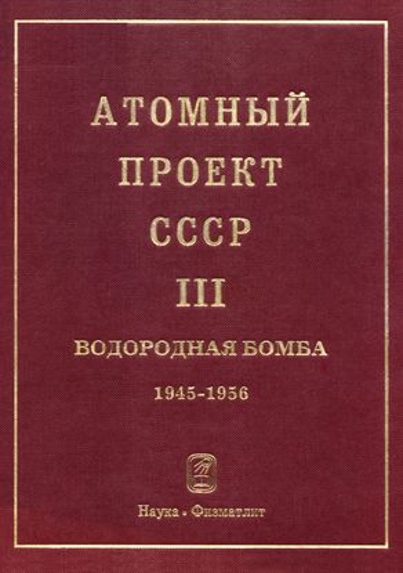
\includegraphics[width=5cm]{pic1}
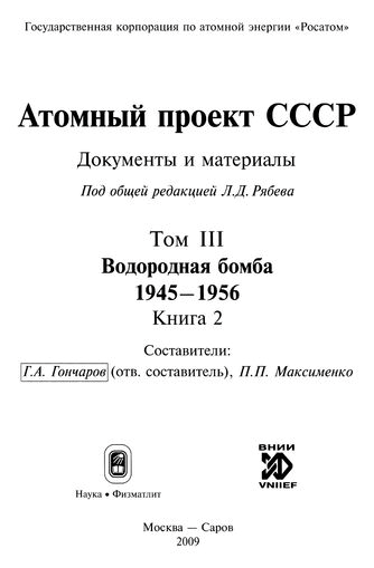
\includegraphics[width=5cm]{pic2}

Но так как труды конференции были уже опубликованы, то эта информация в них не попала. В тоже время, важность этого факта в очередной раз высветила значение С.Г. Крейна не только в воронежской, но и в отечественной математике и заставила нас с новых позиций посмотреть и проследить за теми, иногда неожиданными и судьбоносными человеческими «сцеплениями», благодаря которым наш университет, а вместе с ним и город Воронеж, стали причастными к разработке грандиозного проекта. Этот факт вызвал необходимость публикации дополнения к вышедшим материалам математической школы С.Г. Крейна-2018.

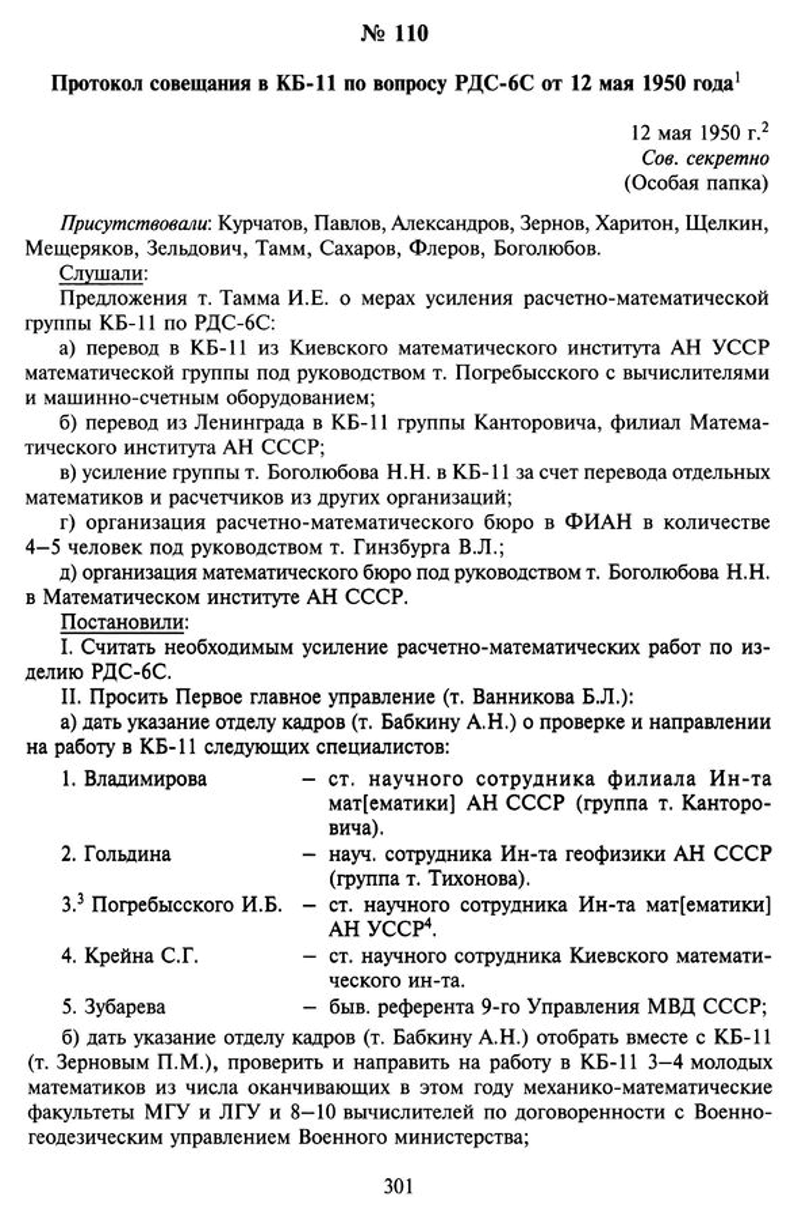
\includegraphics[width=10cm]{pic3}

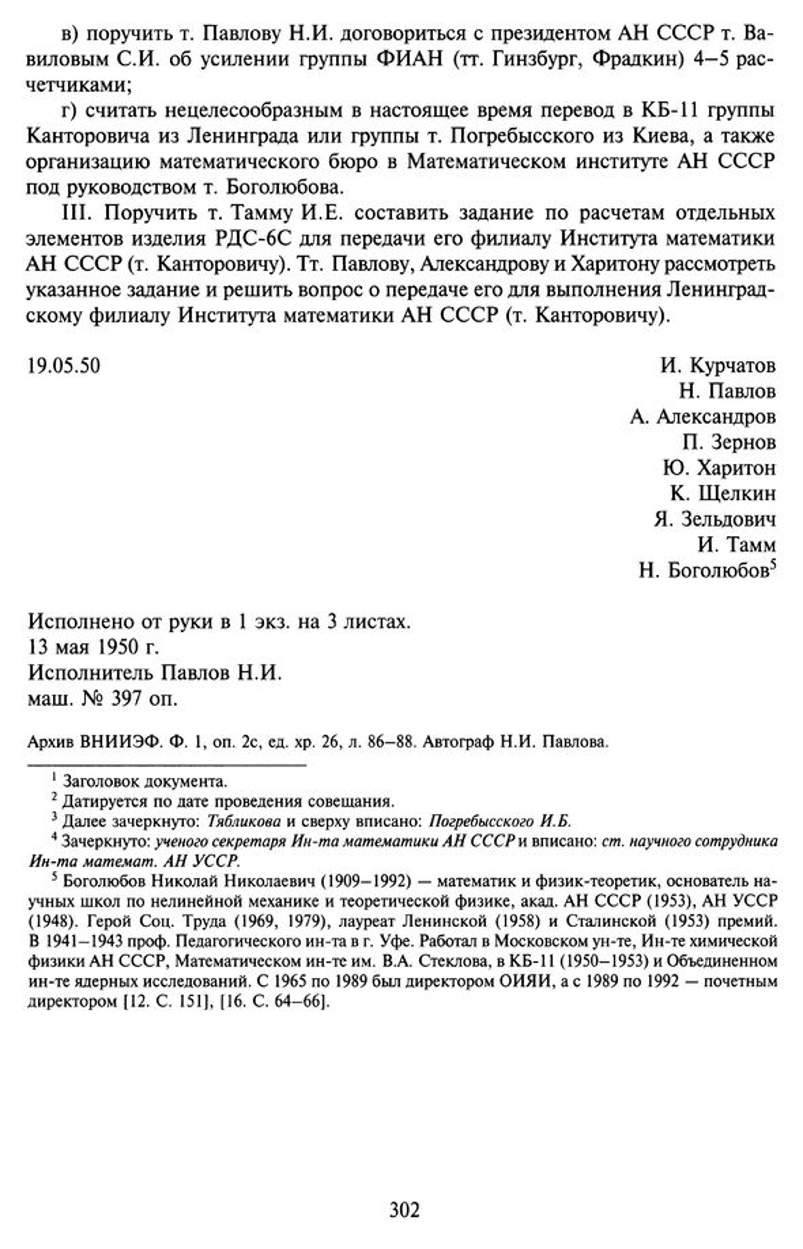
\includegraphics[width=10cm]{pic4}

Может показаться удивительным, но, по мнению авторов, такая «сцепка» начинается с семьи нашего выдающегося земляка – математика А.П. Киселева.

\begin{center}
{\bf А.П. Киселев и А.Д. Билимович}
\end{center}

Имя выдающегося русского педагога нашего земляка воронежца Андрея Петровича Киселева известно многим поколениям учащихся нашей страны. После окончания в 1875 году Санкт-Петербургского университета, где он слушал лекции П.Л. Чебышева, А.Н. Коркина и др., Киселев был назначен преподавателем математики, механики и черчения в Воронежское реальное училище, открывшееся в 1876 году. Здесь началась его работа над созданием его знаменитых учебников, которые выдержали более трёхсот изданий общим тиражом в несколько сотен миллионов экземпляров. Будучи человеком большой эрудиции и широкого кругозора интересов, во время частых поездок заграницу он имел возможность знакомиться с новейшими открытиями в области естествознания, в частности физики, астрономии, медицины. Так, после открытия В. Рентгена, Киселев даже приобрел за границей большую катушку Румкорфа и с ее использованием провел ряд лекций о рентгеновских лучах. Об одной лекции по астрономии рассказывается в воронежской газете «Дон» от 5 января 1892 года: «Публичная лекция „Исследование состава Солнца и других небесных тел посредством спектрального анализа“, прочитанной А.П. Киселевым 2 января в зале реального училища, привлекла массу публики. Этого и надо было ожидать по двум причинам: во-первых, самое содержание лекции небезынтересно для каждого, а во-вторых, симпатичной была самая ее цель "--- воспомоществование пострадавшим от неурожая в Воронежской губернии. Нельзя не выразить искренней благодарности за все старания, которые он приложил к тому, чтобы столь серьезный и важный отдел физики, как спектральный анализ, сделать вполне общедоступным для понимания каждого. Кроме того, все сказанное на лекции обставлялось вполне удавшимися опытами, при помощи электрического света.

 Остается от души пожелать, чтобы подобные лекции повторялись и на будущее время. Они принесли бы, без сомнения, более интереса и пользы, чем оперетки и „отчаянные“ и „раздражительные“ драмы, как, например, „Гетман“, „Две сиротки“ и тому подобная белиберда».

\begin{center}
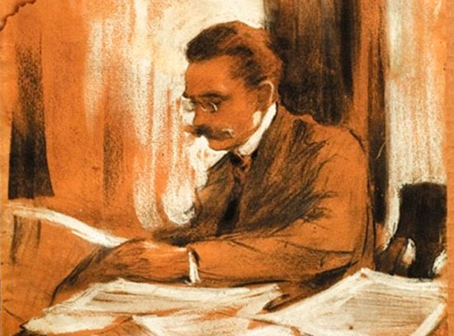
\includegraphics[width=5cm]{pic5}

{\it А.П. Киселев (художник Е.А. Киселева)}
\end{center}


Не удивительно, что находившемуся постоянно в широких научных кругах Андрею Петровичу было суждено породниться и с другим известным российским математиком А.Д. Билимовичем, за которого вышла замуж его дочь Елена Андреевна.

\begin{center}
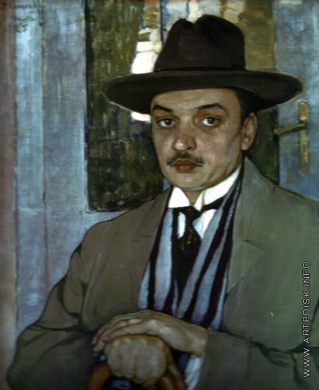
\includegraphics[width=4cm]{pic6}

{\it А.Д. Билимович (художник Е.А. Киселева)}
\end{center}

Билимович Антон Дмитриевич родился 20.06.1879 г. в г. Житомире. В то время Украина входила в состав Российской Империи. Начальную школу окончил в г. Владимире, где служил его отец в качестве военного врача. В 1896 году закончил с отличием Киевский кадетский корпус, а в 1903 г. и физико-математический факультет Киевского университета также с отличием. Оставленный при университете сверхштатным ассистентом, он начал активную научную деятельность. В 1907 г. была опубликована его работа «Приложение геометрических производных к теории кривых и поверхностей», содержавшая систематическое изложение вопросов дифференциальной геометрии в векторной форме.

После защиты магистерской диссертации «Уравнения движения для консервативных систем» (Киев, 1912) Билимович был направлен на стажировку в Париж и в Геттинген. В Париже и произошло знакомство талантливого математика А.Д. Билимовича с талантливой ученицей И.Е. Репина Еленой Киселевой. После женитьбы они в 1914 году вернулись в Россию, где Антон Дмитриевич получил профессорскую должность в Новороссийском университете в Одессе.

В апреле 1915 г. он стал ординарным профессором кафедры прикладной математики Новороссийского университета. На этой должности он читает базовый курс теоретической механики, дополнительные разделы динамики твердого тела, теорию упругости, а также спецкурсы по интегрированию уравнений механики и по теории аэроплана. Одновременно возглавляет механическую мастерскую университета и кабинет механики (1915-1917), продолжает научную работу в области аналитической механики.
После смерти А.\,М.~Ляпунова 3 ноября 1918 г. возглавил комиссию по сохранению, обработке и подготовке к печати работ академика, благодаря чему была сохранена его рукопись «О некоторых фигурах равновесия вращающейся жидкости».
В январе 1920 г. оставил Одессу и вскоре нашел убежище в Сербии, где создал большую научную школу по аналитической механике. Ему также принадлежит заслуга создания в Сербии (в 1920-1960) ряда научных объединений и институтов, участие в издательской деятельности соотечественников-эмигрантов: Российского академического кружка, Российского научного института, двух изданий «Материалов для библиографии русских научных трудов за рубежом», Математического института Сербской Академии наук, открытие которого состоялось в мае 1946г. В 1949 г. вышел первый том «Трудов математического института Сербской Академии наук». Именно в этом издании в течение нескольких лет он печатал свои работы, включая воспоминания «Ляпунов в Одессе» (1956). Кроме того, А. Д. Билимович был одним из основателей Югославского общества механиков.

Научная деятельность была отмечена избранием его 18 февраля 1925 г. членом-корреспондентом, а 17 февраля 1936 г. – действительным членом Сербской Академии наук и искусств.

\begin{center}
{\bf А.Д. Билимович и Н.М. Крылов}
\end{center}

Спустя 48 лет после отъезда из России в неопубликованном письме своей знакомой Нине Александровне от 8.01.1968г. А.Д. Билимович пишет о своем друге Н.М. Крылове.

«В Петрограде у меня был близкий друг Н.М. Крылов, который вместе со мной окончил Киевский кадетский корпус и поступил в Горный институт в Петрограде, нормально окончил и был оставлен при институте профессором математики его учителем математики был проф. Долбня. Крылов уехал заграницу (Париж, Италия, Англия) – и вернулся после революции в Крым, где стал сначала академиком Киевской Академии Наук, а затем и Московской. М.Н. Крылов известен своими работами с Н.Н. Боголюбовым, посвященными так наз. нелинейной механике. При поездках из Киева в Петроград я останавливался у Крылова и встречался у него с многими математиками столицы, но с Андреем Петровичем \textit{(Киселевым "--- прим. авт.)} я тогда знаком не был. Я познакомился с ним только в Югославии, куда он приезжал навестить Владимира Андреевича \textit{(сын Киселева "--- прим. авт.)} преподавателя математики в Белой Церкви и нас, Елену Андреевну, сына Арсения и меня».

\begin{center}
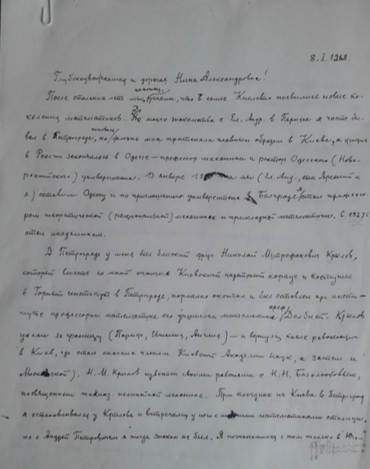
\includegraphics[width=7cm]{pic7}

{\it Фрагмент копии письма А.Д. Билимовича, снятый с одного из экспонатов региональной конференции «Киселевские чтения – 2002», посвященной 150-летию со дня рождения А.П. Киселева, проводимой Воронежским госуниверситетом 16-17 декабря 2002 года}
\end{center}

\begin{center}
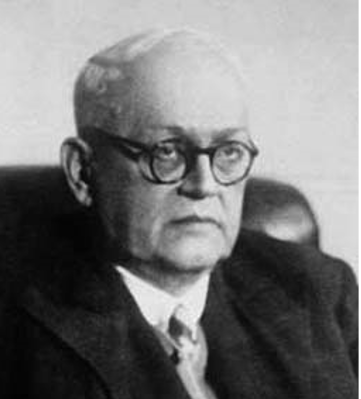
\includegraphics[width=4cm]{pic8}

{\it Н.М. Крылов, академик АН СССР}
\end{center}

Николай Митрофанович Крылов родился 29 ноября 1879 года в Санкт-Петербурге. В 1889 (1890) был принят в Киевский кадетский корпус. Окончил Петербургский горный институт в 1902 году. Позже служил в институте профессором в 1912—1917 годах. В 1917 году переехал в Крым, где до 1922 года служил профессором Крымского университета; с 1917 года также профессор Киевского университета. В 1922-1945 годах возглавлял отдел математической физики АН УССР.

\begin{center}
{\bf Н.М. Крылов и Н.Н. Боголюбов}

\vspace{3mm}

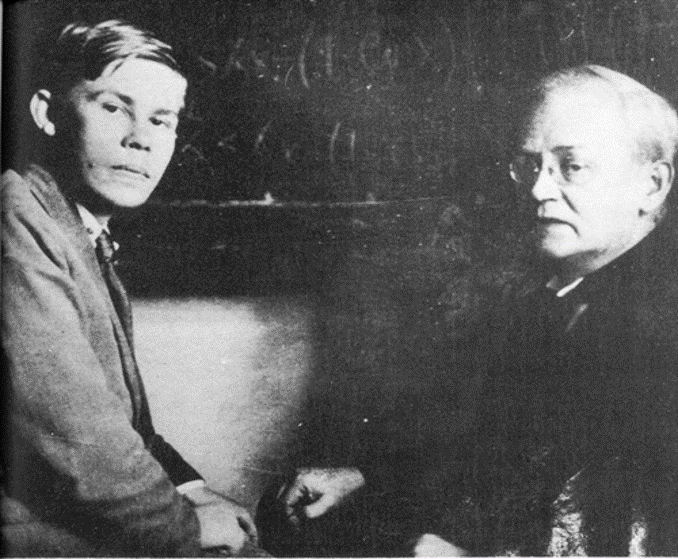
\includegraphics[width=6cm]{pic9}

\end{center}

Эта фотография взята из книги А.Н. Боголюбова о своем старшем брате «Н.Н. Боголюбов. Жизнь. Творчество» (Дубна : ОИЯИ, 1996). На фотографии слева — будущий академик Н.Н. Боголюбов, а справа — его учитель академик Н.М. Крылов. Свою первую научную работу Н.Н. Боголюбов сделал в 15 лет совместно и под руководством Н.М.~Крылова. Несмотря на то, что Н.М. Крылов по образованию был горным инженером, его интересовала математика с точки зрения ее приложений не только в горном деле, но и в самых разных областях природы и техники. Здесь он находил важные задачи и ставил их перед своим учеником.

Будущий академик Николай Николаевич Боголюбов был сыном потомственного священника, профессора богословия Н.М. Боголюбова. У Н.Н. рано проявились математические способности. В 12 лет он самостоятельно, при некотором участии отца, который в молодости также питал влечение к точным наукам, овладел дифференциальным и интегральным исчислением; роль отца заключалась в том, что он снабжал сына необходимой литературой, а впоследствии и сам овладел высшей математикой, чтобы понимать работы сына.

Став учеником Н.М. Крылова, он восемь лет проживал в его квартире. Поэтому Боголюбов был более чем ученик Н.М. Крылова. Он был его воспитанник.

 К 1932 году Н.М. Крылов и Н.Н. Боголюбов создали совершенно новую область математической физики — нелинейную механику. В разработанных ими асимптотических методах, оказавшихся исключительно общими и гибкими, особое внимание было уделено построению простых и эффективных приемов, которые позволили бы, исходя из элементарных соображений, составить приближенные формулы. Предложенные Н.М. Крыловым и Н.Н. Боголюбовым весьма эффективный принцип эквивалентной линеаризации, символические и другие методы существенно облегчили исследования многочисленных нелинейных задач.

\begin{center}
{\bf Н.Н. Боголюбов и С.Г. Крейн}

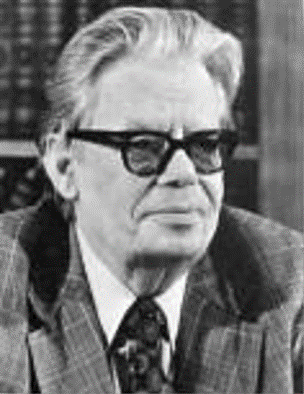
\includegraphics[width=4cm]{pic10}


{\it Н.Н. Боголюбов, академик АН СССР}
\end{center}

Николай Николаевич Боголюбов родился 8 августа 1909 года в городе Нижний Новгород в семье преподавателей Нижегородского Мариинского института благородных девиц.

Начальное образование получил в церковно"=приходской школе, которую окончил в 12 лет. Дальнейшее официальное образование для сына «служителя культа» было невозможным, поэтому отец стал обучать Николая и его младших братьев дома. Благодаря отцу сыновья не только получили обширные знания по истории, философии, лингвистике, литературе, но и унаследовали стремление к интеллектуальному труду. Отец первым заметил у старшего сына талант к точным наукам, особенно к математике и сделал все возможное для его развития.

В 1921 году семья переехала в Киев. Благодаря уникальным математическим способностям юный Николай Боголюбов уже в 14 лет стал полноправным участником семинаров по математике. В 1924 году он познакомился с академиком Н.М. Крыловым, признанным лидером целого направления в математике, членом многих иностранных математических обществ. Уже через год работы с Крыловым Николай опубликовал свою первую математическую работу «О поведении решений линейных дифференциальных уравнений на бесконечности». Исследование оказалось настолько самостоятельным и глубоким, что в 1925 году, в порядке исключения, малый президиум УкрГлавНауки принял решение принять Н.Н. Боголюбова аспирантом на кафедру математики Киевского университета.

В 1928 году (в 19 лет) защитил кандидатскую диссертацию, а в 1930 году Академия наук Украины присудила ему степень доктора математики. С 1928 года — научный сотрудник Института теоретической физики АН УССР (Киев). Работы двадцатидвухлетнего Николая Боголюбова уже получили международную известность, и одна из них была удостоена специальной премии Болонской академии наук.

Нелинейная механика сыграла чрезвычайно важную роль в развитии теории колебаний и многих актуальных разделов техники: радиотехники, теории статической и динамической устойчивости синхронных машин, продольной устойчивости летательных аппаратов и других. Буквально из лаборатории результаты поступали в производство, и уже в первой половине 1930-х годов на базе         нелинейной механики в ряде ведущих технических областей были созданы новые расчетные методы.

В 1936 году молодого профессора впервые направили в научную командировку по Европе, он побывал в Берлине, Париже, Брюсселе.

С началом Великой Отечественной войны киевские академические институты были эвакуированы в Башкирию и Н.Н. Боголюбов оказался в Уфе, где он возглавил кафедры Уфимского авиационного института и Уфимского педагогического института (1941-1943). Кроме того, он продолжил теоретические исследования. Еще перед войной Н.Н. Боголюбов начал работать над проблемой статистических методов в математической физике. Эти исследования он продолжил в Уфе и в 1946 году опубликовал монографию «Проблемы динамической теории в статистической физике».

В начале 1950 года Н.Н. Боголюбов был направлен на «объект» в Сарове (Арзамас-16), где велась работа по созданию ядерного и термоядерного оружия, начальником математического отдела, который затем был преобразован в отделение (cектор).

В это же время, в соответствии с выше приведенным протоколом совещания в КБ-11 по вопросу РДС–6С от 12 мая 1950 года, вместе с ним был переведен и его ученик (аспирант) С.Г. Крейн.

\begin{center}
{\bf М.А. Лаврентьев и С.Г. Крейн}

\vspace{3mm}

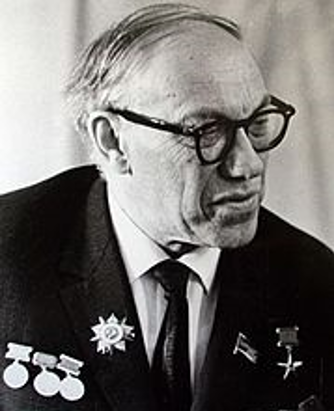
\includegraphics[width=4cm]{pic12}


{\it М.А. Лаврентьев, академик АН СССР}
\end{center}

Михаил Алексеевич Лаврентьев родился 19 ноября 1900 года в семье преподавателя математики технического учебного заведения, позже профессора механики Казанского университета А.Л. Лаврентьева.

В 1910—1911 годах вместе с отцом находился в Гёттингене (Германия), где начал посещать среднюю школу. Среднее образование окончил в Казанском коммерческом училище. В 1918 году поступил в Казанский университет, а в 1921 году перевёлся на физико-математический факультет Московского университета, который окончил в 1922 году. Был оставлен в аспирантуре: в 1923-1926гг. — аспирант Н.\,Н.~Лузина. В 1927 году защитил диссертацию на соискание учёной степени кандидата физико-математических наук и был командирован на полгода во Францию для научного совершенствования.

С 1931 года — профессор МГУ. Без защиты диссертации (по совокупности научных работ) в 1934 году ему была присуждена учёная степень доктора технических наук, а в 1935 году — доктора физико-математических наук.

Во время Великой Отечественной войны  работал в области приложений математики и механики к оборонным вопросам техники и народного хозяйства. Во время эвакуации основного состава Академии наук УССР в Уфу изучал действие на преграду металлического стержня, движущегося с большой скоростью вдоль своей оси. Этим предвосхищается, в сущности, идея кумулятивного действия взрыва, теорией которого М. А. Лаврентьев вплотную занялся в 1944 году. В 1946 году Лаврентьев предложил оригинальную гидродинамическую трактовку явления кумуляции, в соответствии с которой при огромных давлениях, возникающих в момент взрыва, металл можно рассматривать как идеальную несжимаемую жидкость; после этого, используя уравнения гидродинамики, можно было рассчитать динамику струи металла и вычислить пробивной эффект. За работы в области кумуляции Лаврентьев был в 1949 году удостоен Сталинской премии.

Интересны и удивительны научно-технические средства и соответствующие эксперименты, применяемые в научных исследованиях М.А. и его группы, в которую входил и С.Г.  Крейн, при решении такой важной для страны проблемы, как создание кумулятивных снарядов.  Вот что по этому поводу пишет один из членов этой группы доктор технических наук С.В. Малашенко в той же книге.

«Исследуя всесторонне свойства кумулятивной струи, М.А. буквально „сработал“ свои зубы. Опыт требовал — для облицовки внутренней поверхности кумулятивной оболочки снаряда — высокопластичных и особо тяжелых металлов. Уникальная серебряная стопка, уведенная из семейного буфета Веры Евгеньевны, была пущена в дело беспощадно. А мне однажды пришлось переплавить в угольном тигле золотой зубной протез, который М.А. вручил мне со словами: „Я себе другой добуду. Жаль, здесь маловато металла“. „Золотой опыт“ выполнили, результат его показался нам неясным, а М.А., как всегда в таких случаях, глубоко задумался. Дефицитные осесимметричные кумулятивные оболочки стали препятствием для удовлетворения растущих аппетитов в опыте по бронепробиванию. Изобретательный М.А. пустил в ход подручные материалы. Детям приказали яички всмятку есть аккуратно, не разрушая скорлупу полностью. Кумулятивные выемки в форме весьма правильного эллипсоида принесли пользу. Но более эффективной оказалась другая технология. Любимые цветы Веры Евгеньевны (жена М.А.) на подоконнике преждевременно увядали, так как освобожденные от них глиняные конусообразные горшки отлично себя показали при моделировании кумулятивных струй в воде (оболочка типа усеченного конуса). Опыты с применением горшков и вазонов выполнялись в так называемом верхнем „лягушечьем“ пруду. Туда ходили компанией — всегда с гостями. Горшок с закрытым отверстием в дне, с подвязанным внизу зарядом тола отпускался плавать в пруд и там подрывался. Кумулятивная струя была эффектно видна, опыт оценивался по ее высоте („выше осины или выше березы“). Научных результатов в таком опыте было, как правило, два. Гости начинали веровать в наличие особого явления — кумуляции, а М.А. и соучастники опыта с изумлением подтверждали, что лягушки, живущие в пруду, выдерживают действие взрыва. Их выбрасывало на берег, но они были живы».

Лаврентьев и его ученики много внимания уделяли также изучению устойчивости движения твёрдых тел с жидким наполнением с приложением к задачам артиллерии.

Об этом времени М.А вспоминает в книге «Век Лаврентьева»: «Уфа. Военные задачи. Академия наук Украины была переведена в Уфу, туда поехал и я с семьей. Первая зима была самой трудной. Всей семьей из пяти человек жили в гостинице, на шести квадратных метрах. Дети несколько раз болели. Я большую часть времени проводил на работе. Украинской Академии было предоставлено два здания: в одном из них одну комнату занимал Институт математики, где я первый год проводил основную часть времени. Там же работали Н.Н. Боголюбов, С.Г. Крейн, И.З. Штокало, Г.И. Дринфельд. Мы с Крейном занимались проблемой устойчивости снарядов…»


\begin{center}
{\bf С.Г. Крейн и Воронежская математическая школа}

\vspace{3mm}

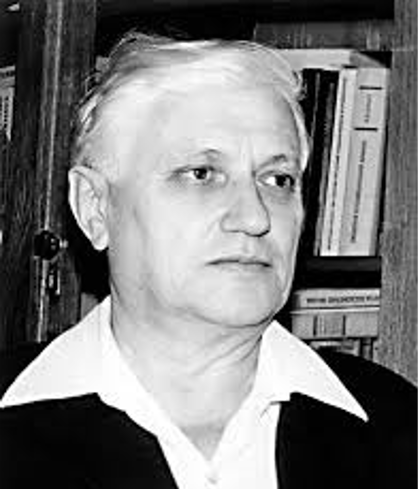
\includegraphics[width=4cm]{pic13}


{\it Селим Григорьевич Крейн, доктор технических наук,
 профессор, заслуженный деятель науки РСФСР}
\end{center}

Является учеником академиков Н.Н. Боголюбова и М.А. Лаврентьева, под руководством которых работал во время Великой Отечественной войны в области приложения математики и механики к оборонным вопросам техники.

С.Г. Крейн родился 15 июля 1917 г. Выдающийся ученый и педагог, крупнейший специалист в области функционального анализа, гидродинамики, дифференциальных уравнений и их приложений, доктор технических наук, профессор, заслуженный деятель науки РФ Селим Григорьевич Крейн большую часть своей жизни (сорок пять лет) отдал созданию и развитию воронежской математической школы. Им опубликовано 175 статей и 18 монографий. Под его руководством было написано 81 диссертация, 24 его ученика стали докторами наук, а двое из них "--- Ю.М.~Березанский и Ю.Л.~Далецкий "--- стали действительными членами АН Украины.

В годы войны Селим Григорьевич под руководством академика М.А. Лаврентьева работал над математическими проблемами теории кумулятивных снарядов. Затем работал в группе академика Боголюбова в КБ-11 по созданию водородной бомбы. В 1950 году в Академии артиллерийских наук защитил диссертацию на соискание степени доктора технических наук.

После войны он возвращается в Киев, а в 1954 году приезжает в Воронеж, где работает в качестве профессора в лесотехническом институте, а с 1964 года – он профессор ВГУ. Ведет чрезвычайно интенсивную научную и педагогическую работу. Круг его интересов очень широк, но основа многих его исследований - функциональный анализ. Вместе с М.А. Красносельским и В.И. Соболевым Селим Григорьевич создает, ставшую хорошо известной в нашей стране и за рубежом, школу функционального анализа.

Ученый. С.Г. Крейн один из первых применил методы функционального анализа к задачам гидродинамики и получил фундаментальные результаты о колебаниях вязкой несжимаемой жидкости. Эти исследования подытожены в монографиях «Операторные методы в линейной гидродинамике» и «Эволюционная теория», написанных совместно с его вьетнамским учеником Нго Зуй Каном и профессором Н.Д. Копачевским.

Вместе с тем, задачи термодинамики привели С.Г. Крейна к необходимости рассматривать в качестве математических моделей дифференциальные уравнения в банаховых пространствах, исследованию корректной и некорректной разрешимости этих задач. Соответствующие исследования были отражены в его классическом труде «Линейные дифференциальные уравнения в банаховом пространстве», вскоре переведенном в США и Японии. Наряду с всемирно известными французскими математиками Э. Гальярдо, Ж. Лионсом, А. Кальдероном Селим Григорьевич является создателем современной теории интерполяции линейных операторов. Предложенный им метод шкал банаховых пространств нашел широкое применение как в теории операторов, так и в теории дифференциальных уравнений. По этим исследованиям совместно с его учениками Ю.И. Петуниным и Е.М. Семеновым написана монография «Интерполяция линейных операторов», переведенная в США.

Организатор. В 1967 году по его инициативе С.Г. Крейна и под его руководством впервые в Воронеже была проведена зимняя математическая школа, вскоре ставшая популярной и оказавшая большое влияние на развитие контактов между математиками из разных городов и стран. В связи с идеей создания школы, приведем слова Селима Григорьевича, характеризующие масштабы его интересов и планов, направленных на развитие воронежской математики: «В 1966 году в Москве проходил Международный съезд математиков. Наряду с яркими впечатлениями от многих докладов и бесед с известными зарубежными математиками (Филлипс, Иосида, Кальдерон, Комацу и д.р.) у меня осталось чувство неудовлетворенности. Мне показалось, что у нас имеется по ряду направлений отставание от современного на тот момент уровня».

Так появилась и захватила идея проведения зимних математических школ, в которых читались лекции и делались доклады по самым современным проблемам математики как ведущими учеными, так и молодыми математиками.


\begin{center}

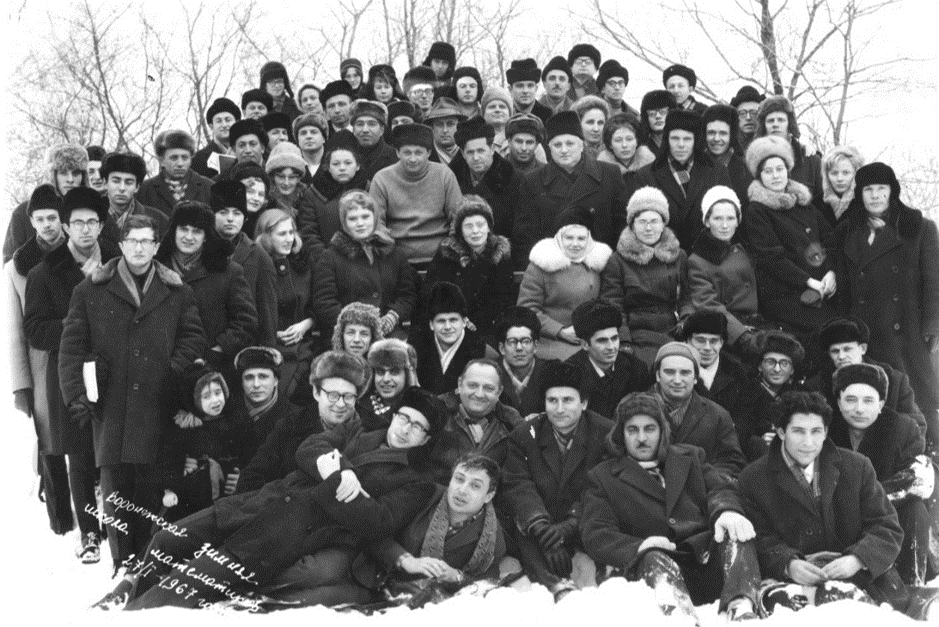
\includegraphics[width=10cm]{pic14}


{\it Первая воронежская зимняя математическая школа (ВЗМШ)
27 января 1967 года. Дом отдыха им. Горького}
\end{center}

Трудно переоценить значение математических разговоров и дискуссий между участниками школы. Иногда до поздней ночи работали небольшие внеплановые «самодеятельные» семинары. По словам С.Г. Крейна: «В школе нет выборов, нет премий, нет демократии, поэтому работа проходит в спокойной, творческой обстановке. Молодые математики очень легко воспринимают новые идеи и смело начинают их использовать. Мы тоже, по мере сил, пытались „задрав штаны, бежать за комсомолом“».

В разные годы лекторами и активными участниками ВЗМШ были выдающиеся математики, ученые с мировым именем: академики РАН С.П. Новиков, В.И. Арнольд, В.П.~Маслов, А.Т. Фоменко, чл.-кор. Укр. Академии Наук Ю.М. Березанский и чл.-кор. Укр. Академии Наук Ю.Л.~Далецкий.

В частности, были прочитаны лекции: В.И. Арнольд «Топопология алгебраических многообразий», В.П. Маслов «Функции от некоммутирующих операторов и их применение». А.Т. Фоменко выступал с курсами лекций на темы «Минимальные поверхности и проблема Плато», «Многомерные вариационные задачи», «Топологическая классификация интегрируемых гамильтоновых систем».

В настоящее время школа получила международный статус.  Ее бессменными руководителями, начиная с 2006 года, являются академики РАН В.П. Маслов – председатель оргкомитета и А.Т. Фоменко – председатель программного комитета.

\begin{center}

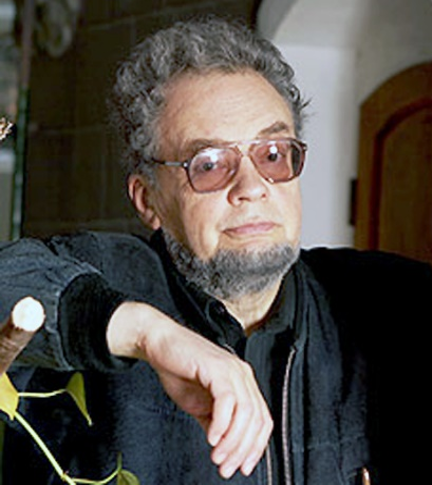
\includegraphics[width=5cm]{pic15}


{\it Виктор Павлович Маслов, академик АН СССР}
\end{center}

{\it Выдающийся специалист в области математической физики, дифференциальных уравнений, функционального анализа, механики и квантовой физики.

С 1992 г. по 2016 г., вслед за Н.Н. Боголюбовым, возглавлял кафедру квантовой статистики и теории поля в МГУ.  Н.Н. Боголюбов и С.Г. Крейн были оппонентами при защите докторской диссертации Маслова на тему «Теория возмущений и асимптотические методы». Разработал асимптотические методы, широко применяемые к уравнениям, возникающим в квантовой механике, теории поля, статистической физике, абстрактной математике, и носящие его имя. Асимптотические методы Маслова тесно связаны с такими проблемами, как теория самосогласованного поля в квантовой и классической статистике, сверхтекучесть и сверхпроводимость, квантование солитонов, квантовая теория поля в сильных внешних полях и в искривленном пространстве-времени, метод разложения по обратному числу типов частиц.

Занимался проблемами жидкости и газа, проводил фундаментальные исследования по проблемам магнитной гидродинамики, связанным с проблемой динамо.

В 1986 г. руководил группой экспертов-математиков, участвовавших в создании проекта захоронения аварийного блока Чернобыльской АЭС. О ситуации на АЭС в монографии «Математическое моделирование аварийного блока Чернобыльской АЭС» В.П. Маслов с соавторами пишут: «Драматическая обстановка аварии и осознанная ответственность за обоснованность выводов и рекомендаций обусловливали, несмотря на сжатые сроки исполнения, особенно тщательный и беспристрастный анализ всей совокупности полученных данных». Здесь весьма важно подчеркнуть, что, несмотря на чрезвычайность ситуации, был применен строго научный подход решения конкретных задач с использованием фундаментальных исследований.  В указанной монографии говорится: «Хотя уравнения модели являются классическими, новый тип краевых задач для них привел к открытию новых физических эффектов, которые позволили последовательно объяснить важные особенности в поведении аварийного реактора».

С начала 90-х годов работал над использованием уравнений математической физики в экономике и финансовом анализе. При расчетах использовались уравнения, аналогичные уравнениям фазового перехода в физике.

Автор более 300 научных работ, в том числе 12 монографий.

Государственная премия СССР (1978), Золотая медаль им. А.М. Ляпунова (1982), Ленинская премия (1985), дважды лауреат Государственной премии РФ (1997, 2013), Демидовская премия (2000).}

\begin{center}

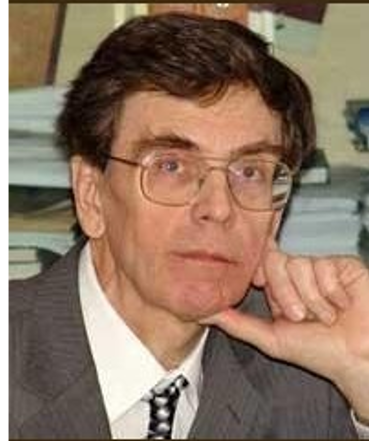
\includegraphics[width=4cm]{pic16}


{\it Анатолий Тимофеевич Фоменко, академик АН СССР}
\end{center}

{\it Родился в 1945 году. Академик Российской Академии Наук (РАН), доктор физико-математических наук, профессор, зав. кафедрой механико-математического факультета Московского государственного университета.

Выдающийся специалист в области многомерного вариационного исчисления, дифференциальной геометрии, теории групп и алгебр Ли, симплектической и компьютерной геометрии. Действительный член общественных организаций «Российская академия естественных наук» и «Международная академия наук высшей школы». Автор нескольких книг по разработке и применению новых эмпирико-статистических методов к анализу исторических летописей, хронологии древности и средневековья.

А.Т. Фоменко хорошо известен в научном мире как оригинальный художник-график. Избранная коллекция его работ, любезно подаренная им Воронежскому государственному университету, является бесценным экспонатом университетского музея. Эту грань многогранного таланта он успешно использует в разработке математических методов познания окружающего мира через геометрические образы. По этому поводу в интервью Российской Философской газете (№6 [20] июнь 2008) А.Т. Фоменко говорит, что эти работы были сделаны для целей математики – для чтения спецкурса и для иллюстраций математических книг, т.е. для лучшего донесения до студентов и аспирантов математических теорем.  Он подчеркивает: «Дело в том, что в топологии и геометрии очень много сложных конструкций, которые обычно трудно объяснять, причём для доказательства теорем часто не только пишут формулы (иногда это не просто), но и используют «жаргон», наглядные образы. …Графические работы оказались полезны для преподавания, вызвали интерес и у студентов, и у математиков. Потом по просьбе коллег я стал делать иллюстрации для гидродинамики, для теории вероятностей».

Автор более 200 научных работ, 30 монографий и учебников.

Лауреат Государственной Премии РФ в области математики (1966) за цикл работ по теории многообразий и гамильтоновых динамических систем.}


\begin{center}

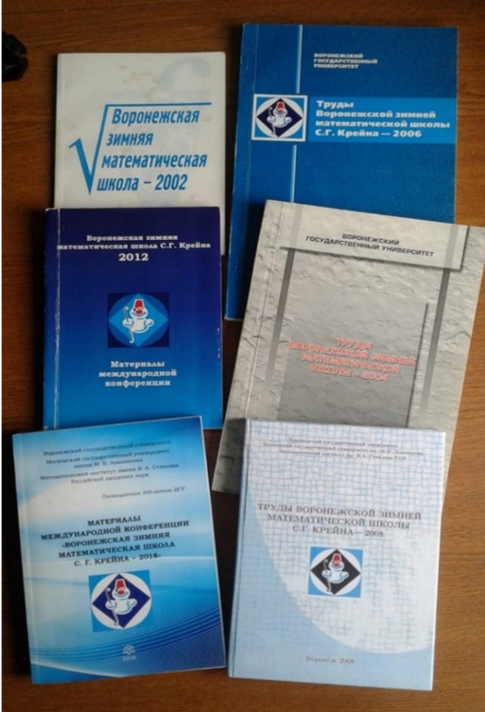
\includegraphics[width=6cm]{pic17}


{\it Хранители ценностей
«крейновских» математических школ
}
\end{center}

Опыт проведения «крейновских» зимних математических школ с успехом распространился и на другие регионы. Так, в последнее время зимние математические школы по теории функций и функциональному анализу проводятся в Воронеже по нечетным годам, а по четным годам – в Саратове, под руководством академика Б.С. Кашина и поддерживаемые грантами РФФИ.

\begin{center}

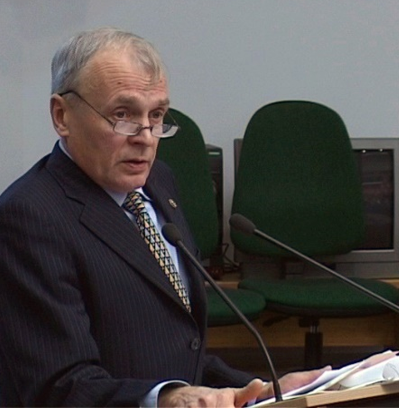
\includegraphics[width=5cm]{pic18}


{\it Борис Сергеевич Кашин, академик РАН
}
\end{center}


{\it Родился в 1951 году. Доктор физико-математических наук, зав. кафедрой теории функций и функционального анализа мехмата МГУ, Действительный член Академии Наук РФ.

 Специалист в области ортогональных рядов, теории аппроксимации, геометрии выпуклых тел. Полученный Кашиным важный результат в теории выпуклых тел лег в основу нового метода обработки сигнала «сжатые измерения», получивший важные практические приложения. Монография Кашин Б. С., Саакян А. А.  Ортогональные ряды. 2-е изд. — М.: Изд-во АФЦ, 1999. 550 с. — ISBN 5-93379-003-6.}


\begin{center}

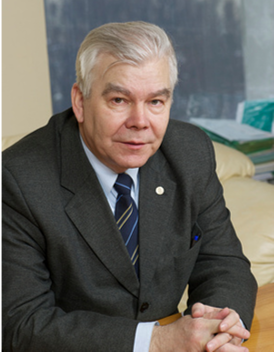
\includegraphics[width=3cm]{pic19}


{\it Евгений Иванович Моисеев, академик РАН
}
\end{center}

{\it
Родился в 1948 году. Российский физик и математик, профессор, академик РАН (2003).

Область научных интересов: информатика, математическое моделирование, спектральная теория, дифференциальные уравнения. Получены фундаментальные результаты в теории задач для уравнений смешанного типа в газовой динамике, в теории турбулентной плазмы. Развиты разностные методы решения краевых задач, возникающих в теории турбулентности и плазмы. Совместно с академиком В.А. Ильиным выполнен большой цикл работ по оптимизации граничного управления колебания струны.

Автор свыше 120 научных работ.
}

В 1966 году у С.Г. Крейна возникла идея создания в ВГУ научно-исследовательского института математики. Он пишет: «Когда меня уговаривали стать деканом, то в качестве одного из условий, я поставил оказание ректором помощи в организации института. Такая помощь была обещана». Но, так как организация института не значилась ни в каких планах нашего планового хозяйства, то Селиму Григорьевичу пришлось пройти много испытаний, прежде чем институт был открыт. Например, С.Г. в двухдневный срок пришлось для Госплана по науке и технике написать перспективный план развития института по 16-ти научным направлениям. Поддержку Академии Наук СССР ускорил академик Н.Н.~Боголюбов. И институт математики был открыт 30      ноября 1967 года.
На волне моды на эконометрику, поднявшуюся в следствии присуждения Нобелевской премии по экономике академику Л.В.~Канторовичу, с которым С.Г. был близок, при его активном участии была открыта экономическая лаборатория, которая позже была преобразована в экономический институт под руководством В.Н.~Эйтингона. Благодаря активной деятельности Крейна были открыты на математико-механическом факультете следующие кафедры: кафедра уравнений с частными производными и теории вероятностей, а кафедра вычислительной математики и кафедра математических методов в экономике, по существу, заложили основы факультета прикладной математики и механики, открывшемуся в 1969 году.
К числу созидательных дел, свершившихся также благодаря Крейну, нужно отнести и создание кафедры математического моделирования, 20-летие которой мы отмечаем в настоящем 2018 году.


\begin{center}

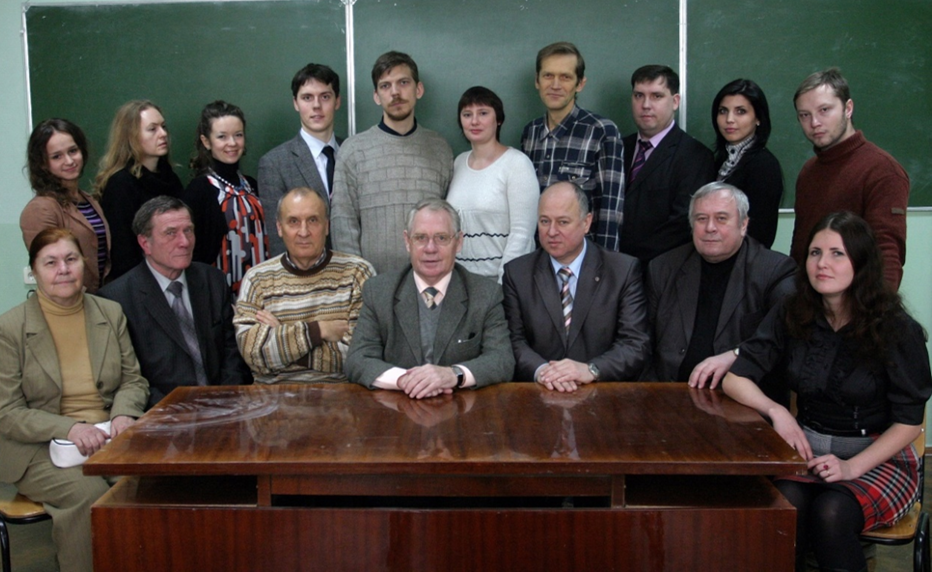
\includegraphics[width=10cm]{pic20}


{\it Кафедра математического моделирования (2009).

Слева направо. Сидят: Г.Б. Савченко, В.Г. Фирсов, В.Г. Орлов, В.А. Костин (зав. кафедрой), А.А. Чаплыгин, Ю.И. Сапронов, А.П. Карпова. Стоят: М. Малюгина, Н.А. Ярцева, Т.И. Костина, Д.В. Костин, С.Л. Царев, Н.Б. Подтынникова, С.М. Семенов, А.В. Костин, М.Н. Небольсина, А. Борзаков
}
\end{center}

Являясь председателем ГЭК на математическом факультете, в 1983 году Крейн сразу высоко оценил и поддержал увлечение математикой молодого инженера-конструктора Сергея Валюхова, уже окончившего к тому времени с красным дипломом Московское Бауманское училище и работающего на космическом предприятии КБ Химавтоматики, созданном знаменитым советским конструктором С.А. Косбергом.


\begin{center}

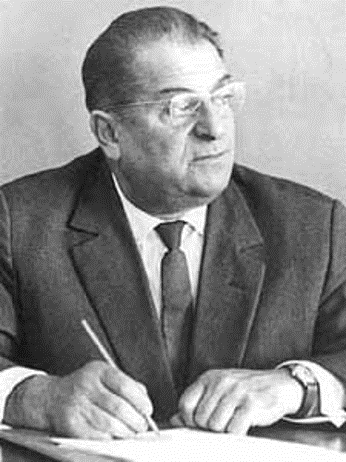
\includegraphics[width=4cm]{pic21}


{\it Семен Ариевич Косберг}
\end{center}

{\it С.А. Косберг (1903–1965 гг.) – знаменитый авиаконструктор. Венцом его многочисленных конструкторских достижений является создание третьей ступени ракеты Р-7, позволившей развить вторую космическую скорость. Именно эта ступень обеспечила вывод аппарата Ю.А. Гагарина на орбиту. Когда это произошло, Юрий Гагарин, забыв о требовании секретности, открытым текстом сообщил миру: «Косберг включился!» Семен Ариевич трагически погиб в автомобильной катастрофе 3 января 1965 года на обледенелой ВОГРЭСовской дамбе.

Его именем назван кратер на обратной стороне Луны.
}

Понимая особое значение математики в решении стоящих перед космическим производством задач, Сергей Валюхов нашел необходимым получить более глубокие знания по математике, успешно закончив математический факультет воронежского университета.
 Позже С.Г. Валюхов поддержал идею создания на факультете сначала лаборатории, а затем и кафедры математического моделирования, при этом оказав помощь как в направлении научной тематики, так и финансовую.


\begin{center}

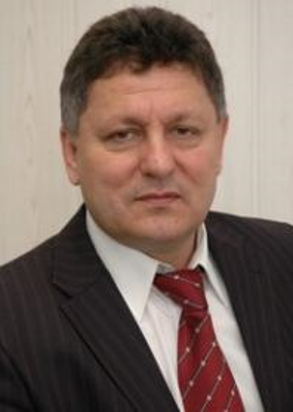
\includegraphics[width=4cm]{pic22}


{\it Сергей Георгиевич Валюхов}
\end{center}

{\it Родился в 1953 году. Доктор технических наук, профессор, генеральный конструктор, генеральный директор АО «Турбонасос» (г. Воронеж), заведующий кафедрой нефтегазового оборудования и транспортировки Воронежского государственного технического университета, Академик Российской Инженерной академии.}

В 1983 году начались наши научные контакты с КБ Химавтоматика. Они проходили в рамках хоздоговоров по кафедре функционального анализа. Но уже в начале девяностых годов С.Г. Валюхов вместе со своим отделом выделился в самостоятельную организацию «Турбонасос».  С этого момента наши связи стали постоянно расширяться и углубляться. Перед нами ставились актуальные и важные, с производственной точки зрения, задачи. В то же время они были новыми и интересными для нас, так как фундаментальные математические исследования реализовывались в конкретном производственном процессе. Сюда относятся исследования по геометрии винтовых шестеренчатых зацеплений, теории движения жидкости в гидроциклоне, задачи по теории гидроцепей и многое другое.
К этому времени у нас сформировался исследовательский коллектив единомышленников. Стал вопрос о создании учебно-научной лаборатории, которая была открыта в 1997 году при полной финансовой поддержке со стороны предприятия «Турбонасос». Оставался последний шаг к созданию кафедры. И он был сделан уже через год. Так, в 1998 году в ВГУ родилась кафедра математического моделирования (КММ), освященная делами и идеями выдающихся наших современников С.Г. Крейна, С.А. Косберга.

\begin{center}
{\bf Ученики С.Г. Крейна}
\end{center}

По данным Американского Математического общества на 2003 год первое место в мире по количеству учеников, имеющих ученую степень за все времена, занимает воронежский математик С.Г. Крейн, опережая таких выдающихся математиков современности, как Д. Гильберт и А.Н. Колмогоров.

Доктора физ.-мат. наук

\noindent 1.	акад. Академия Наук УССР \par Березанский Юрий Макарович (г. Киев)

\noindent 2.	акад. Академия Наук УССР \par Далецкий Юрий Львович (г. Киев)

\noindent 3.	Петунин Юрий Иванович (г. Киев)

\noindent 4.	Копачевский Николай Дмитриевич (г. Симферополь)

\noindent 5.	Панков Александр Андреевич (США)

\noindent 6.	Павлов Евгений Александрович (г. Луганск)

\noindent 7.	Соболевский Павел Евсеевич (Израиль)

\noindent 8.	Кучмент Петр Абрамович (США)

\noindent 9.	Нго Зуй Канн (Вьетнам)

\noindent 10.	 Фам Ки Ань (Вьетнам)

\noindent 11.	 Зайденберг Михаил Григорьевич (Франция)

\noindent 12.	 Глушко Владимир Павлович (г. Воронеж)

\noindent 13.	 Семенов Евгений Михайлович (г. Воронеж)

\noindent 14.	 Седаев Александр Андреевич (г. Воронеж)

\noindent 15.	 Овчинников Владимир Иванович (г. Воронеж)

\noindent 16.	 Курина Галина Алексеевна (г. Воронеж)

\noindent 17.	 Чернышов Корнелий Исидорович (г. Воронеж)

\noindent 18.	 Костин Владимир Алексеевич (г. Воронеж)

\noindent 19.	 Зарубин Анатолий Георгиевич (г. Хабаровск)

\noindent 20.	 Фролов Николай Николаевич (г. Владивосток)

\noindent 21.	 Лаптев Геннадий Иванович (г. Тула)

\noindent 22.	 Зубова Светлана Петровна (г. Воронеж)

\noindent 23.	 д. тех. н. Сысоев Юрий Семенович (г. Волгодонск)

\noindent 24.	 д. тех. н. Поличка Нина Петровна (г. Хабаровск)

                     Кандидаты физ.-мат. наук

\noindent  1.	Костарчук Виктор Николай (г. Чернигов)

\noindent  2.	Артемов Георгий Абрамович (г. Севастополь)

\noindent  3.	Духовный Михаил Сергеевич (г. Кривой Рог)

\noindent  4.	Шихватов Александр Александрович (г. Николаев)

\noindent  5.	Козлов Овсей Маркович (г. Киев)

\noindent  6.	Якут Лидия Ивановна (г. Киев)

\noindent  7.	Ярошенко Николай Степанович (г. Киев)

\noindent  8.	Кведерас Брюнюс Винцевич (г. Вильнюс)

\noindent  9.	Аскеров Назим Кафарович (г. Баку)

\noindent  10.	Ливчак Алексей Яковлевич (г. Рига)

\noindent  11.	Нгуен Ши Хонг   (Вьетнам)

\noindent  12.	Чан Тху Ха (Вьетнам)

\noindent  13.	Зобин Наум Михайлович (США)

\noindent  14.	Львин Сергей Яковлевич (США)

\noindent  15.	Грабовская Маргарита Яковлевна (США)

\noindent  16.	Товбис Александр Исаакович (Австралия)

\noindent  17.	Рутицкая Алла Яковлевна (Австралия)

\noindent  18.	Николова Людмила (Болгария)

\noindent  19.	Николов Красемир (Болгария)

\noindent  20.	Беляева Елена Владимировна (Н.Зеландия)

\noindent  21.	Литминков Степан Сергеевич (г. Воронеж)

\noindent  22.	Прозоровская Ольга Ивановна (г. Воронеж)

\noindent  23.	Иевлева Оксана Борисовна (г. Воронеж)

\noindent  24.	Шаблицкая Лилия Нколаевна (г. Воронеж)

\noindent  25.	Складнев Сергей Анатольевич (г. Воронеж)

\noindent  26.	Гудович Николай Николаевич (г. Воронеж)

\noindent  27.	Руссман Асаак Борисович (г. Воронеж)

\noindent  28.	Савченко Юлия Борисовна (г. Воронеж)

\noindent  29.	Трофимов Валерий Павлович (г. Воронеж)

\noindent  30.	Колупанова (Цветкова) Галина Андреевна (г. Воронеж)

\noindent  31.	Гудович (Титиевская) Ирина Семеновна (г. Воронеж)

\noindent  32.	Иванов Леонид Александрович (г. Воронеж)

\noindent  33.	Штейнберг Иосиф Яковлевич (г. Воронеж)

\noindent  34.	Салехов Дмитрий Васильевич (г. Воронеж)

\noindent  35.	Котко Людмила Антоновна (г. Воронеж)

\noindent  36.	Фурменко Александр Иванович (г. Воронеж)

\noindent  37.	Савченко Галина Борисовна (г. Воронеж)

\noindent  38.	Дементьева Ольга Владимировна (г. Воронеж)

\noindent  39.	Зюкин Павел Николаевич (г. Воронеж)

\noindent  40.	Горохов Евгений Владимирович (г. Воронеж)

\noindent  41.	Сапронов Иван Васильевич (г. Воронеж)

\noindent  42.	Копанева Вера Ивановна (г. Воронеж)

\noindent  43.	Гохман Алексей Оскарович (Канада)

\noindent  44.	Атласов Игорь Викторович (г. Воронеж)

\noindent  45.	Веневитина Светлана Семеновна (г. Воронеж)

\noindent  46.	Куликов Иван Михайлович (г. Борисоглебск)

\noindent  47.	Денисов Игорь Васильевич (г. Тула)

\noindent  48.	Симонов Александр Сергеевич (г. Тула)

\noindent  49.	Осипов Валерий Борисович (г. Владивосток)

\noindent  50.	Кседзенко Людмила Степановна (г. Владивосток)

\noindent  51.	Гасанов Насир Мелекович (г. Махачкала)

\noindent  52.	Дмитриев Вячеслав Иванович (г. Курск)

\noindent  53.	Яцкин Николай Иванович (г. Иваново)

\noindent  54.	Брыскин Илья Борисович (Израиль)

\noindent  55.	Плющев Юрий Васильевич (г. Сергиев Посад)

\noindent  56.	Чубарин Юрий Павлович (г. Ижевск)

\noindent  57.	Пененсон Исаак Залманович (США)

\noindent  58.	Фомин Василий Иванович (г. Тамбов)

\noindent  59.	Соломатина Любовь Евгеньевна (г. Москва)


\litlist

1.	Атомный проект СССР: документы и материалы : в 3 т. Т. 3. Водородная бомба. 1945–1956. Кн. 2. / под общ. ред. Л. Д. Рябева ; Гос. корпорация по атом. энергии «Росатом»; отв. сост. Г. А. Гончаров. – Саров : РФЯЦ-ВНИИЭФ~; М. : ФИЗМАТЛИТ, 2009. – 600 с.

2.	Моргулис А. Законодатель школьной математики / А.~Моргулис, В. Тростников // Наука и жизнь. – 1968. – № 1.~– С. 121.

3.	Професоры Одеського (Новоросiйского) унiверситету~: биограф. словарь:  в 4 т. Т. 1. Ректори / ОНУ iм. I. I. Мечникова, Науч.б-ка. – 2-ге вид., доп. – Одеса : Астропринт, 2005. – С. 66–69.

4.	История отечественной математики 1917–1967~: в 4~т.~/ Академия наук СССР, Академия наук УССР. – Киев~: Наукова думка, 1970. – Т. 4, кн. 2. – С. 668.

5.	Боголюбов А. Н. Николай Митрофанович Крылов / А. Н. Боголюбов, В. М. Урбанский. – Киев : Наук. думка, 1987. – С. 178.

6.	Малашенко С.В. И тогда он встал к станку. Век Лаврентьева: сб. статей / С.В. Малашенко – Новосибирск : Издательство СОРАН, 2000. –  С. 94–100.

7.	Маслов В. П. Воспоминания о Н. Н. Боголюбове. Воспоминания об академике Н. Н. Боголюбове. К 100-летию со дня рождения : сб. статей / В. П. Маслов. – М. : МИАН, 2009. – 178 с.

8.	Фоменко А. Т. Как было на самом деле. Каждая история желает быть рассказанной / А. Е. Фоменко. – М. : АСТ, 2017. – 788 С.
9.	Костин В.А.  С. Г. Крейн. Воспоминания учеников и коллег / В. А. Костин (отв. ред.), Б. Н. Садовский, Е. М. Семенов. – Воронеж : Издательско-полиграфический центр ВГУ, 2008. – С. 151.

10.	Костин В. А. Ученый. Учитель. Кумир / В. А. Костин~// Воронежский университет. – 2012. – 17 сент. – № 16 (2488).

11.	Костин В. Воронежская зимняя математическая школа С. Г. Крейна – 2008 / В. Костин, В. П. Маслов, В. И. Овчинников, Ю. И. Сапронов, Е. М. Семенов, В. Т. Титов, А. Т. Фоменко // Вестник РФФИ. – 2008. – № 2 (58). – С.~24-26.

12.	Шаракшанэ С. История + математика = научная революция? / С. Шаракшанэ / Российская философская газета. – 2008. – № 6 (20).

